\section{Fonctionnalités supplémentaires d'ADTool}
    \label{sec:ADTool}
    Cette section décrit la conception des fonctionnalités qui vont être ajoutées à ADTool afin de le rendre plus ergonomique.
    
    \subsection{Annulation des dernières actions}
    	La {\sc Figure}~{\ref{fig:ctrlz}} illustre l'agencement des classes permettant de réaliser la fonctionnalité d'annulation d'ADTool. Tout d'abord, chaque action annulable possède sa propre classe définissant l'action à exécuter, ainsi que l'action opposée permettant de l'annuler. Par exemple, les actions permettant d'ajouter un nœud-fils, de changer le label d'un nœud ou encore d'ajouter un paramètre possèdent leurs classes respectives \emph{AddChildEdit}, \emph{ChangeLabelEdit} et \emph{AddDomainEdit}. Ces dernières travaillent toutes sur un ADTree, représenté ici par une classe \emph{ADTree} pour simplifier le diagramme. Ces classes implémentent également \emph{UndoableEdit}, l'interface générique d'une action annulable. Enfin, un gestionnaire d'actions \emph{HistoryManager} stocke les actions effectuées dans un attribut, tout en disposant de méthodes permettant d'annuler ces actions dans l'ordre inverse de celui de leur réalisation.
    	
    	\begin{figure}[H]
	        \centering
	        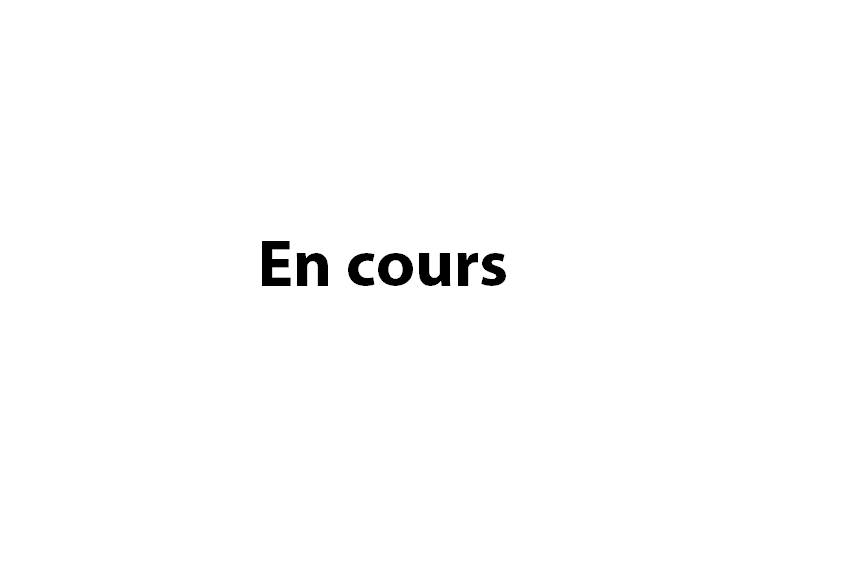
\includegraphics[height=0.8\textwidth]{figure/ctrlz.png}
	        \caption{Diagramme de classes de l'annulation des dernières actions.}
	        \label{fig:ctrlz}
	    \end{figure}
    
    \subsection{Couper-copier-coller}
		La {\sc Figure}~{\ref{fig:copiercoller}} illustre le diagramme de classes permettant d'implémenter le couper-copier-coller dans ADTool. Les ADTrees, représentés par la classe \emph{ADTree}, implémentent \emph{Transferable}, l'interface permettant à un élément d'être coupé, copié ou collé. ADTool, schématisé par la classe \emph{ADTool}, se voit doté d'un \emph{ADTreeTransfertHandler}, une classe permettant de réaliser les actions couper-copier-coller en elles-mêmes. \emph{ADTreeTransfertHandler} implémente \emph{TransfertHandler}, l'interface qui permet de gérer un \og presse-papier \fg{}. Ce dernier est représenté par la classe \emph{Clipboard}, et contient l'élément coupé ou copié, c'est-à-dire un ADTree.
    	
    	\begin{figure}[H]
	        \centering
	        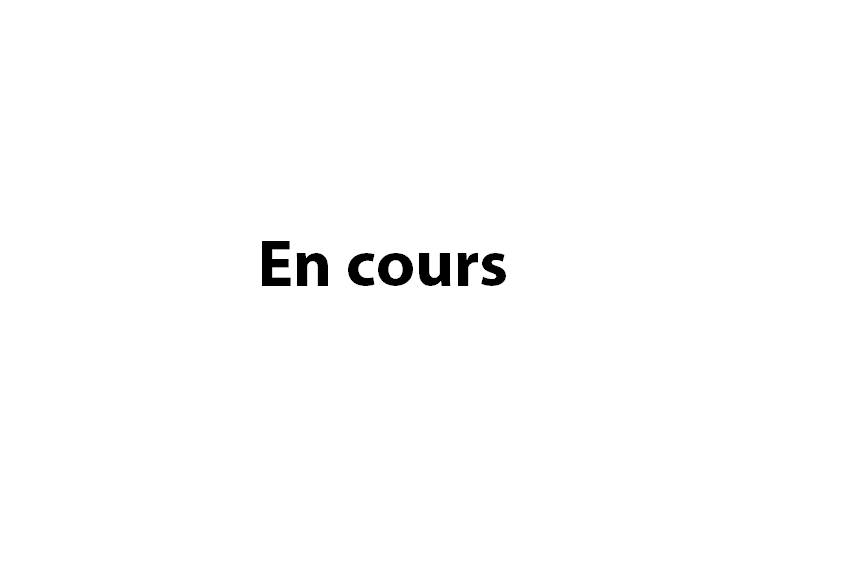
\includegraphics[height=0.6\textwidth]{figure/copiercoller.png}
	        \caption{Diagramme de classes du couper-copier-coller.}
	        \label{fig:copiercoller}
	    \end{figure}
	    
	\subsection{Vue globale des paramètres}

		 La vue globale permet de présenter un condensé de l'ensemble des paramètres présents sur un ADTree. En effet, actuellement, chaque paramètre est affiché dans un onglet, ce qui ne permet pas d'avoir une vision de toutes les valuations en un seul coup d'œil. Il est donc nécessaire d'appliquer quelques changement d'affichage pour offrir à l'utilisateur un aperçu simple et condensé de toutes les valuations d'un nœud.
	
		L'affichage d'un ADTree sous ADTool se fait au moyen des fonctions de la classe \emph{ADTreeCanvas}. Ces fonctions utilisent une autre classe de ADTool, \emph{DomainCanvas}, qui gère l'affichage des paramètres. Comme toutes les valuations de chacun des noeuds d'un ADTree sont présentes dans son fichier XML, nous allons gèrer l'affichage simultané de plusieurs paramètres en détectant avec les fonctions de \emph{ADTreeCanvas} le nombre de paramètres de l'ADTree à afficher, et en appelant autant de \emph{DomainCanvas} lors de l'affichage.
	
	\subsection{Amélioration de la représentation textuelle}

		Pour rappel, ADTool dispose d'une zone d'édition dans laquelle l'ADTree courant est montré sous forme textuelle. La grammaire employée dans cette fenêtre n'est pas tout à fait complète, et mérite donc d'être améliorée. Pour illustrer cela, nous allons utiliser comme exemple l'ADTree de la {\sc Figure}~\ref{fig:arbre_ex}.

		\begin{figure}[H]
	        \centering
	        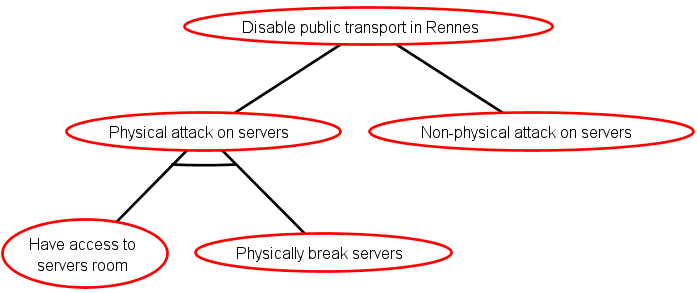
\includegraphics[height=0.4\textwidth]{figure/tree.png}
	        \caption{ADTree servant d'exemple pour illustrer l'amélioration de la zone textuelle.}
	        \label{fig:arbre_ex}
	    \end{figure}

	    L'ADTree de la {\sc Figure}~\ref{fig:arbre_ex} est ainsi actuellement représenté textuellement dans ADTool par le texte de gauche sur la {\sc Figure}~\ref{fig:grams}. On constate l'absence des labels des nœuds pères des différentes opérations (conjonction ou disjonction). Or, ces labels sont primordiaux pour avoir une bonne compréhension de l'ADTree, et surtout pour avoir la totalité des informations qu'il contient. C'est pourquoi nous souhaiterions les rajouter, d'une façon semblable à celle présentée sur la partie droite de la {\sc Figure}~\ref{fig:grams}.

	    \begin{figure}[H]
	        \centering
	        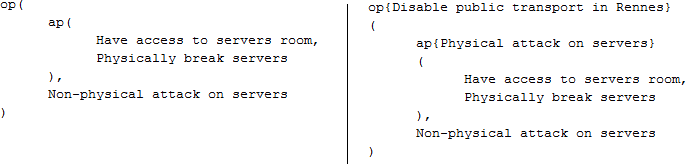
\includegraphics[width=\textwidth]{figure/grams.png}
	        \caption{La grammaire actuelle (à gauche) et la grammaire améliorée (à droite).}
	        \label{fig:grams}
	    \end{figure}

		Pour réaliser ces changements et améliorer la lisibilité de la zone textuelle, il va falloir modifier deux fichiers d'ADTool :
		\begin{itemize}
		\item \emph{ADTNode.java}, la classe représentant un nœud au sein d'un ADTree ;
		\item \emph{adtparser.jit}, le fichier générant la zone textuelle en elle-même.
		\end{itemize}
		
		À travers ces deux fichiers, il est possible de modifier la grammaire régissant la représentation textuelle des ADTrees.